\chapter{Distributed Hash Tables}
\begin{figure}[htbp]
   \centering
   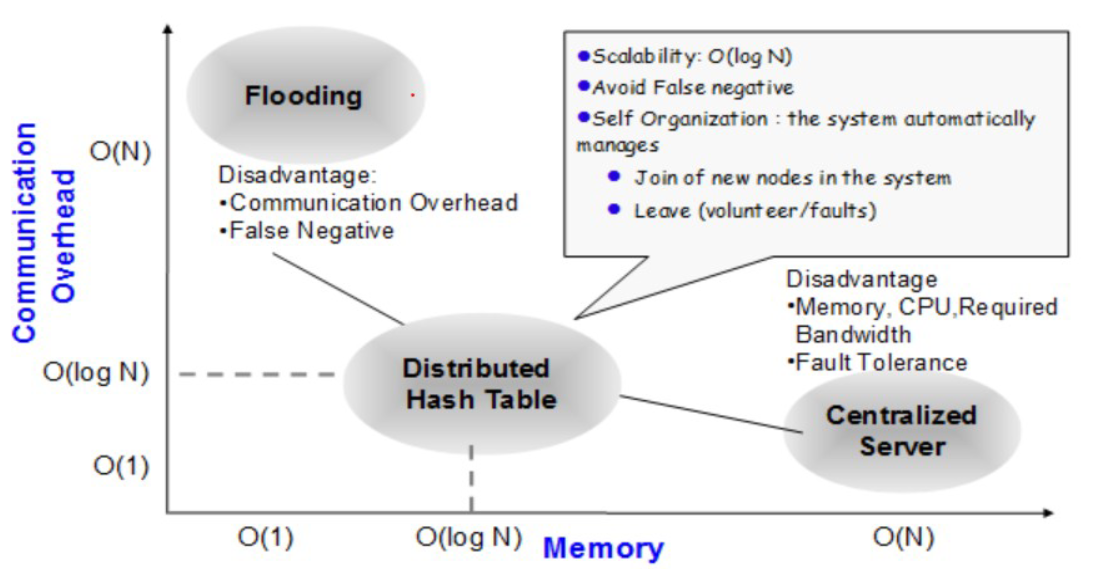
\includegraphics{images/DHT_motivations.png}
   \caption{DHT Motivations}
   \label{fig:DHT_motivations}
\end{figure}

The key idea is to split the hash tables into several parts and distribute them to several servers, and to use hash of resources (or of the URLs of resources) as a key to map them to a
dynamically changing set of web caches, but with \ul{each key mapped to single server}; so that
each machine (user) can locally compute which web cache should contain the
required resource, refenced by an URL.\\
This technique is extended to DHT for P2P systems.

However, \ul{\textbf{rehashing} is a problem in dynamic scenarios} if the hashing scheme depends directly on the number of servers:
$99\%$ of keys have to be remapped, resulting in a lot of messages exchange.
\begin{figure}[htbp]
   \centering
   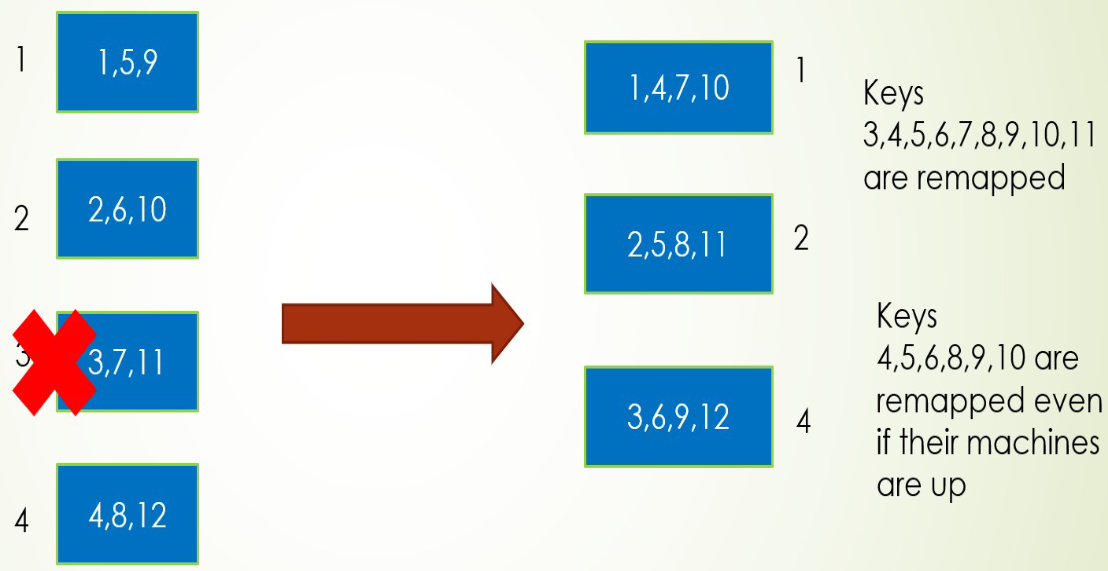
\includegraphics{images/rehashing_problem.png}
   \caption{Rehashing problem}
   \label{fig:rehashing_problem}
\end{figure}

\textbf{Consistent hashing} is a set of hash techniques which guarantees that adding more nodes/remove nodes implies \ul{moving only a minority of data items}.
each node manages ---instead of a set of sparse keys--- an interval of consecutive hash keys, and intervals are joined/splitted when nodes join/leave the network and keys redistributed between adjacent peers.


\section{Building DHT}
\begin{paracol}{2}
   % \colfill
   \begin{itemize}
      \item Use a logical name space, called \textit{identifier space} consisting of identifiers
      $\{0,1,2,...,N-1\}$
      \item define identifier space as a \textit{logical ring} modulo $N$
      \item every node picks a random identifier
      through Hash $H$.
   \end{itemize}
   \begin{figure}[htbp]
      \centering
      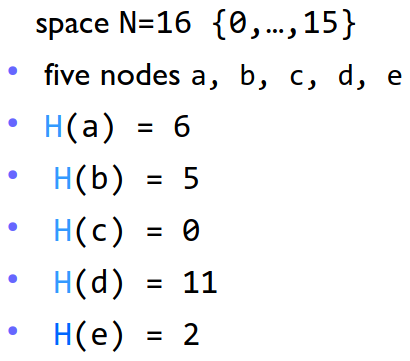
\includegraphics{images/DHT_build2.png}
      % \caption{}
      \label{fig:DHT_build2}
   \end{figure}

   % \colfill
   \switchcolumn
   
   % \begin{adjustbox}{valign=\fill}
   \begin{figure}[htbp]
      \centering
      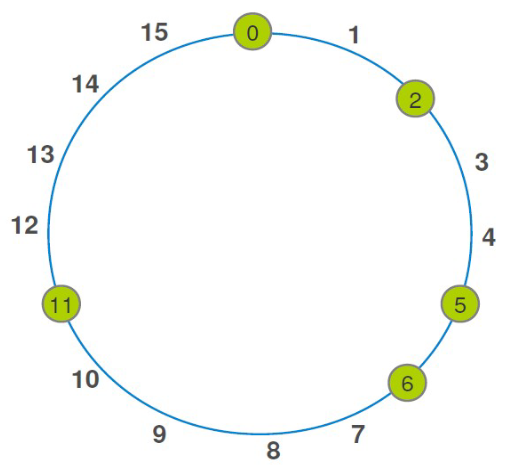
\includegraphics{images/DHT_build1.png}
      \caption{Identifier space}
      \label{fig:DHT_build1}
   \end{figure}
   % \end{adjustbox}
   
\end{paracol}

\subsection{Peers joining and leaving}
When a new node is \textbf{added}, we map the keys between the new node and the previous node in the hash ring to point to the new node;\\
those the keys will no longer be associated with their old nodes.

When a node is \textbf{removed} from the hash ring, only the keys associated with that node are rehashed and remapped rather than remapping all the keys.

In case a node suddenly disconnects from the network, all data stored on it are lost if they are not stored on other nodes;
to avoid such a problem:
\begin{itemize}
   \item introduce some redundancy (data replication)
   \item information loss: periodical information refresh
\end{itemize}

\begin{figure}[htbp]
   \centering
   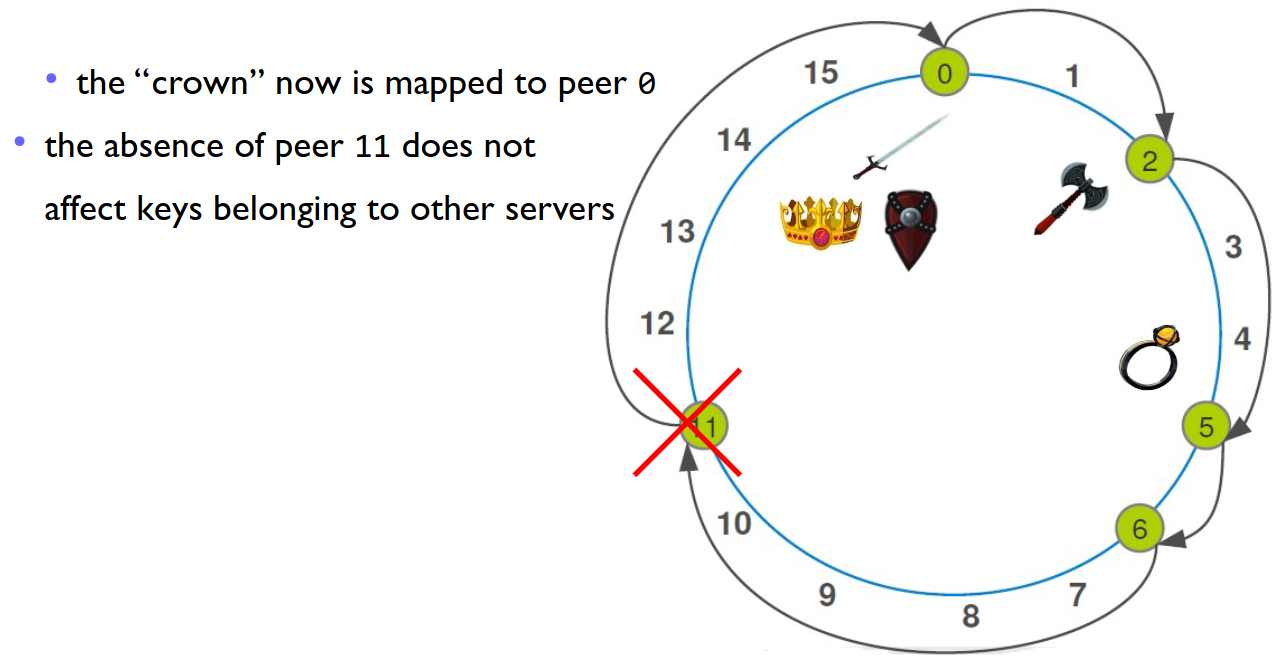
\includegraphics{images/p2p_peerleaves.png}
   \caption{Peer 11 leaves the Network}
   \label{fig:p2p_peerleaves}
   In case a peer leaves, its keys can easily be remapped to its successor
\end{figure}

When the hash table is \textbf{resized}, on the average,only $\frac{k}{n}$ keys need to be remapped on average, where $k$ is the number of keys and $n$ is the number of servers.
\newpage
\section{Data Lookup}
\begin{figure}[htbp]
   \centering
   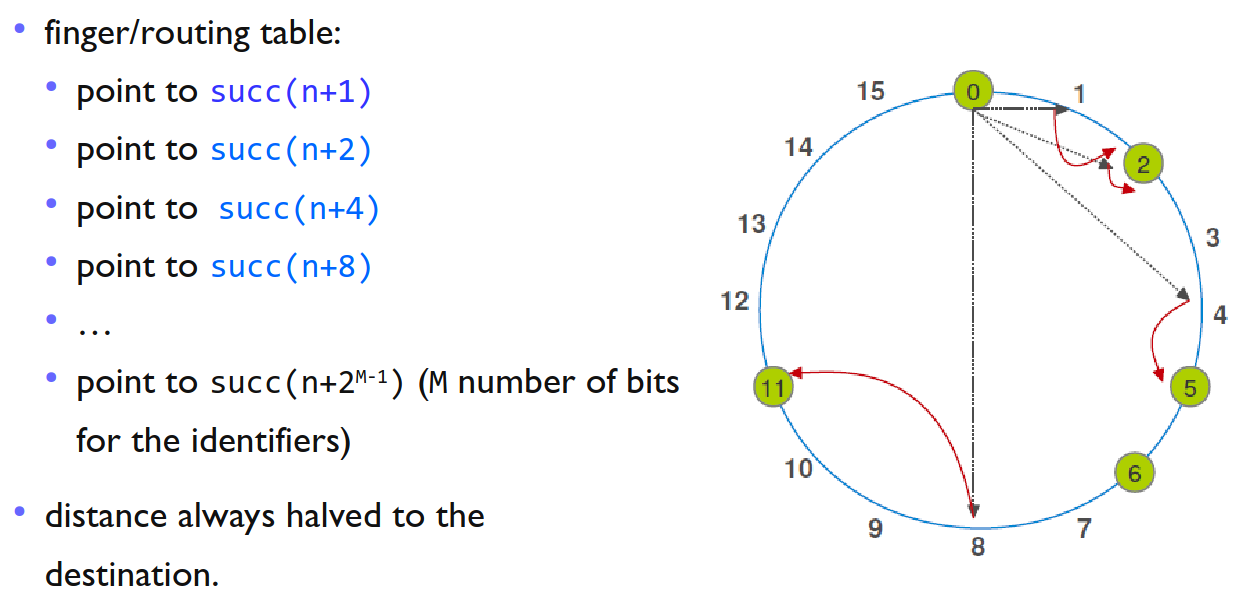
\includegraphics{images/dht_exponentialsearch.png}
   \caption{Exponential Search for DHT}
   The data lookup can be implemented by using exponential search, rather than performing a walk by asking each peer for its successor
   \label{fig:dht_exponentialsearch}
\end{figure}

Data Lookup can be sped up even more, by computing the hash $h(x)$ of the searched object, and propagating the query to farthest node\footnote{Which is found using exponential search} which has an identifier smaller than $h(x)$, which then recursively applies the same algorithm, until the object is found.
\begin{figure}[htbp]
   \centering
   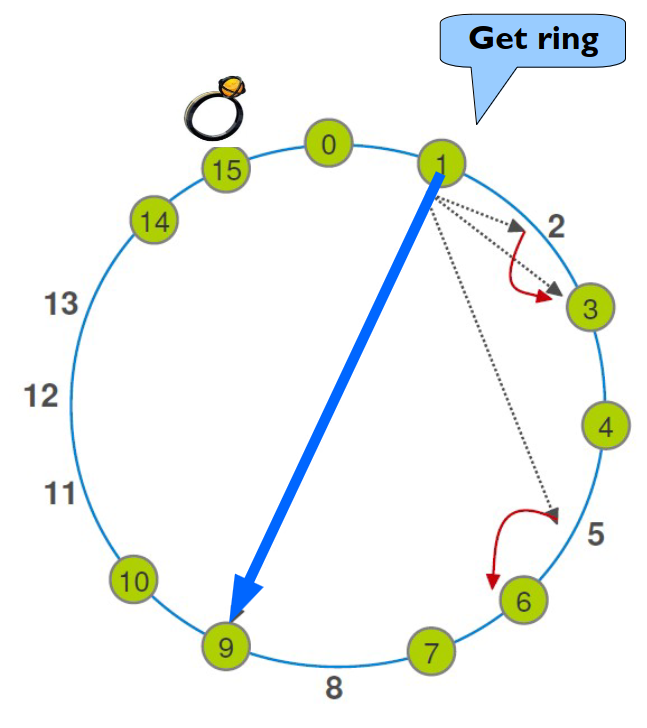
\includegraphics[width=0.3\columnwidth]{images/dht_chordsearch01.png}
   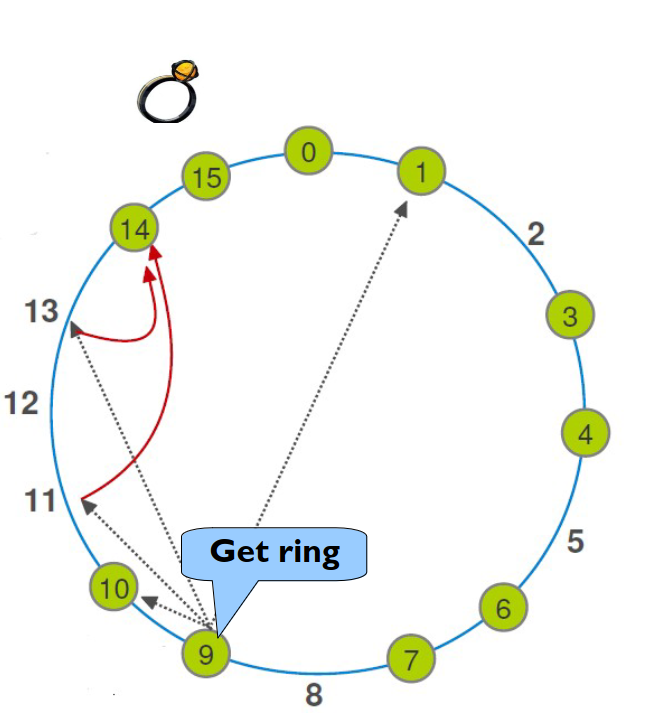
\includegraphics[width=0.3\columnwidth]{images/dht_chordsearch02.png}\\
   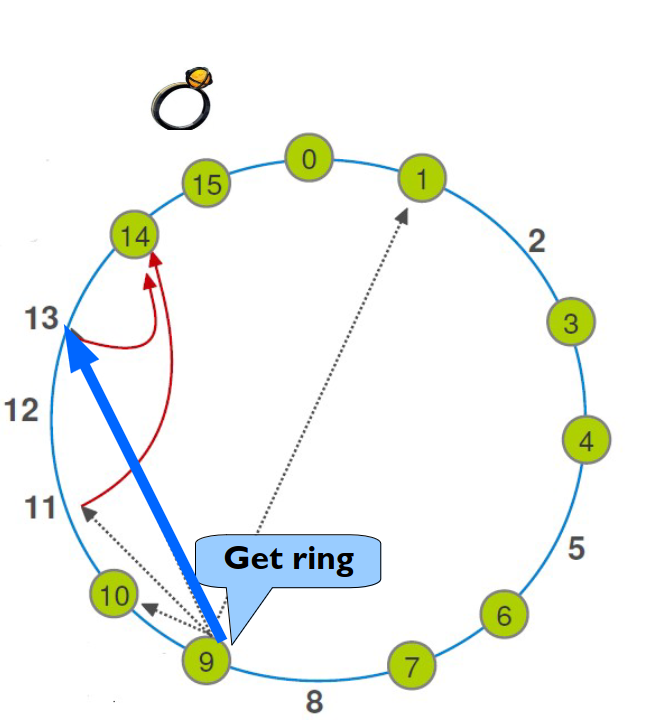
\includegraphics[width=0.3\columnwidth]{images/dht_chordsearch03.png}
   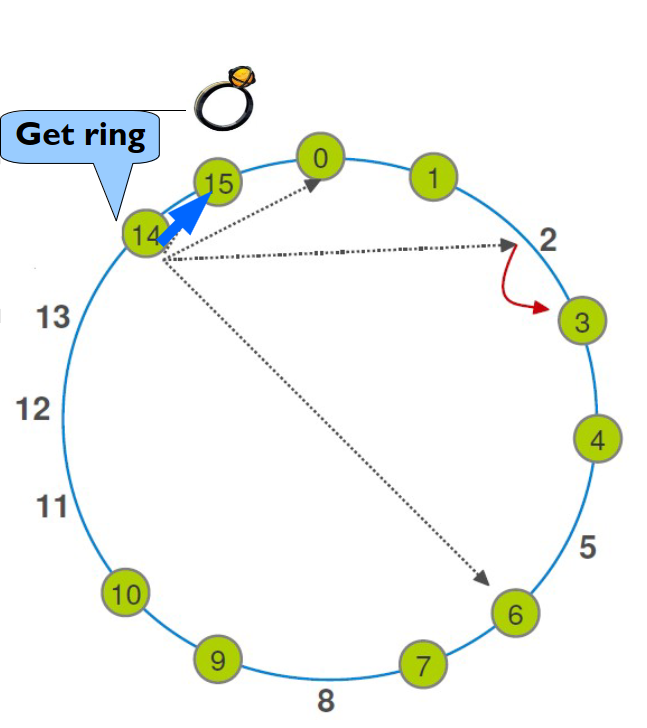
\includegraphics[width=0.3\columnwidth]{images/dht_chordsearch04.png}
   \caption{Lookup performed in the \texttt{\textbf{CHORD}} DHT}
   \label{fig:dht_chordsearch}
\end{figure}

TODO integrate notes from February $28^th$